\chapter{Phân tích yêu cầu và nghiệp vụ}

\section{Phân tích tác nhân (Actors)}

Hệ thống phục vụ ba nhóm người dùng chính là giảng viên, học viên và quản trị
viên. Bên cạnh đó, một số tác nhân hệ thống như LMS, AI Pipeline và LLM
Provider được mô hình hóa riêng vì chúng tham gia trực tiếp vào các luồng
nghiệp vụ.

\begin{table}[H]
    \centering
    \caption{Danh sách tác nhân của hệ thống.}
    \label{tab:actors}
    \begin{tabular}{p{3.5cm}p{10.5cm}}
        \toprule
        \textbf{Tác nhân} & \textbf{Mô tả} \\
        \midrule
        Giảng viên & Người tạo khóa học, upload tài liệu, review nội dung AI và publish cho học viên. \\
        Học viên & Người học nội dung đã publish, làm quiz và tìm kiếm nội dung liên quan. \\
        Quản trị viên & Người quản lý tài khoản, cấu hình hệ thống, theo dõi vận hành và chi phí. \\
        LMS & Nền tảng bên ngoài như Open edX hoặc Moodle, khởi tạo LTI launch và truyền context người dùng. \\
        AI Pipeline & Tác nhân hệ thống xử lý tài liệu, sinh embedding, card, quiz và đồng bộ dữ liệu. \\
        LLM Provider & Dịch vụ mô hình ngôn ngữ được gọi để sinh nội dung hoặc phân tích tri thức. \\
        \bottomrule
    \end{tabular}
\end{table}

Vòng đời nghiệp vụ chính bắt đầu khi giảng viên đưa tài liệu vào hệ thống.
AI Pipeline xử lý tài liệu bất đồng bộ, sinh nội dung nháp, sau đó giảng viên
review và publish. Học viên chỉ tương tác với nội dung đã được công bố và kết
quả học tập được lưu lại để phục vụ phản hồi, thống kê và định hướng adaptive
learning về sau.

\section{Yêu cầu hệ thống}

\subsection{Yêu cầu nghiệp vụ}

\begin{longtable}{|p{1.5cm}|p{4cm}|p{8.5cm}|}
    \caption{Yêu cầu nghiệp vụ (BR).} \label{tab:br-lvtn} \\
    \hline
    \textbf{ID} & \textbf{Tên} & \textbf{Mô tả} \\
    \hline
    \endfirsthead
    \hline
    \textbf{ID} & \textbf{Tên} & \textbf{Mô tả} \\
    \hline
    \endhead

    BR-01 & Xác thực và phân quyền &
    Hệ thống phải phân biệt giảng viên, học viên và quản trị viên; mỗi vai trò chỉ được truy cập chức năng phù hợp. \\ \hline

    BR-02 & Quản lý tài liệu học tập &
    Giảng viên có thể đưa tài liệu vào hệ thống, theo dõi xử lý, review và công bố nội dung. \\ \hline

    BR-03 & Sinh nội dung AI có kiểm soát &
    Hệ thống tự động sinh card/quiz nhưng nội dung phải được kiểm duyệt trước khi học viên nhìn thấy. \\ \hline

    BR-04 & Gắn kết chuẩn đầu ra &
    Nội dung và câu hỏi cần liên kết với Learning Outcome khi có đề cương môn học. \\ \hline

    BR-05 & Tích hợp LMS &
    Hệ thống phải hoạt động như công cụ học tập bên ngoài thông qua LTI, không phụ thuộc vào một LMS duy nhất. \\ \hline

    BR-06 & Theo dõi học tập &
    Hệ thống cần lưu tiến độ học, kết quả quiz và dữ liệu phục vụ phân tích học tập. \\ \hline
\end{longtable}

\subsection{Yêu cầu chức năng}

\begin{longtable}{|p{1.5cm}|p{4cm}|p{8.5cm}|}
    \caption{Yêu cầu chức năng (FR).} \label{tab:fr-lvtn} \\
    \hline
    \textbf{ID} & \textbf{Nhóm chức năng} & \textbf{Mô tả} \\
    \hline
    \endfirsthead
    \hline
    \textbf{ID} & \textbf{Nhóm chức năng} & \textbf{Mô tả} \\
    \hline
    \endhead

    FR-01 & Xác thực & Hỗ trợ đăng nhập nội bộ và LTI launch từ LMS; lưu session an toàn phía server. \\ \hline
    FR-02 & Upload tài liệu & Nhận file PDF/DOCX/PPTX, kiểm tra kích thước/định dạng, lưu object storage và tạo document metadata. \\ \hline
    FR-03 & Xử lý bất đồng bộ & Enqueue job, cập nhật trạng thái pipeline và retry lỗi tạm thời. \\ \hline
    FR-04 & Parsing và chunking & Trích xuất văn bản/cấu trúc, chia chunk theo heading hoặc fallback chunking. \\ \hline
    FR-05 & Embedding và tìm kiếm & Sinh embedding cho chunk, lưu Qdrant và hỗ trợ semantic search top-K. \\ \hline
    FR-06 & Sinh card/quiz & Gọi LLM để sinh summary, lesson card, quiz, đáp án đúng và giải thích. \\ \hline
    FR-07 & Curriculum extraction & Trích xuất course, chapter, LO, assessment từ đề cương môn học. \\ \hline
    FR-08 & LO-aware quiz & Sinh quiz theo LO/chapter/assessment, có Bloom level và rationale. \\ \hline
    FR-09 & Review/publish & Giảng viên xem, sửa, xóa, thêm và publish nội dung sau khi review. \\ \hline
    FR-10 & Learning experience & Học viên xem card, làm quiz, nhận phản hồi và lưu tiến độ. \\ \hline
    FR-11 & Admin/observability & Quản trị viên xem log, trạng thái job, cấu hình provider và thống kê chi phí. \\ \hline
\end{longtable}

\subsection{Yêu cầu phi chức năng}

\begin{longtable}{|p{1.5cm}|p{4cm}|p{8.5cm}|}
    \caption{Yêu cầu phi chức năng (NFR).} \label{tab:nfr-lvtn} \\
    \hline
    \textbf{ID} & \textbf{Tên} & \textbf{Tiêu chí} \\
    \hline
    \endfirsthead
    \hline
    \textbf{ID} & \textbf{Tên} & \textbf{Tiêu chí} \\
    \hline
    \endhead

    NFR-01 & Hiệu năng & API đọc card/quiz mục tiêu P95 $\leq$ 500ms trong môi trường staging; pipeline xử lý tài liệu 20 trang mục tiêu $\leq$ 3 phút. \\ \hline
    NFR-02 & Khả dụng & Giao diện responsive, thông báo lỗi rõ, người dùng không cần thao tác kỹ thuật khi pipeline lỗi tạm thời. \\ \hline
    NFR-03 & Bảo mật & Session/token không lộ ra client không cần thiết; LTI launch xác thực JWT/OIDC; API key lưu qua biến môi trường. \\ \hline
    NFR-04 & Tin cậy & Pipeline idempotent ở mức job/document; lỗi tạm thời retry có giới hạn; lỗi cuối cùng lưu trạng thái \texttt{ERROR}. \\ \hline
    NFR-05 & Bảo trì & Use case không phụ thuộc trực tiếp vào adapter hạ tầng; có unit test cho domain/application. \\ \hline
    NFR-06 & Mở rộng & Có thể thêm parser, embedder, LLM provider, vector DB hoặc LMS integration thông qua adapter. \\ \hline
    NFR-07 & Đánh giá được & Hệ thống lưu đủ metadata để đánh giá retrieval, chất lượng quiz, latency và tỷ lệ lỗi. \\ \hline
\end{longtable}

\section{Phân tích Use Case}

\subsection{Biểu đồ Use Case tổng quát}

\begin{figure}[H]
    \centering
    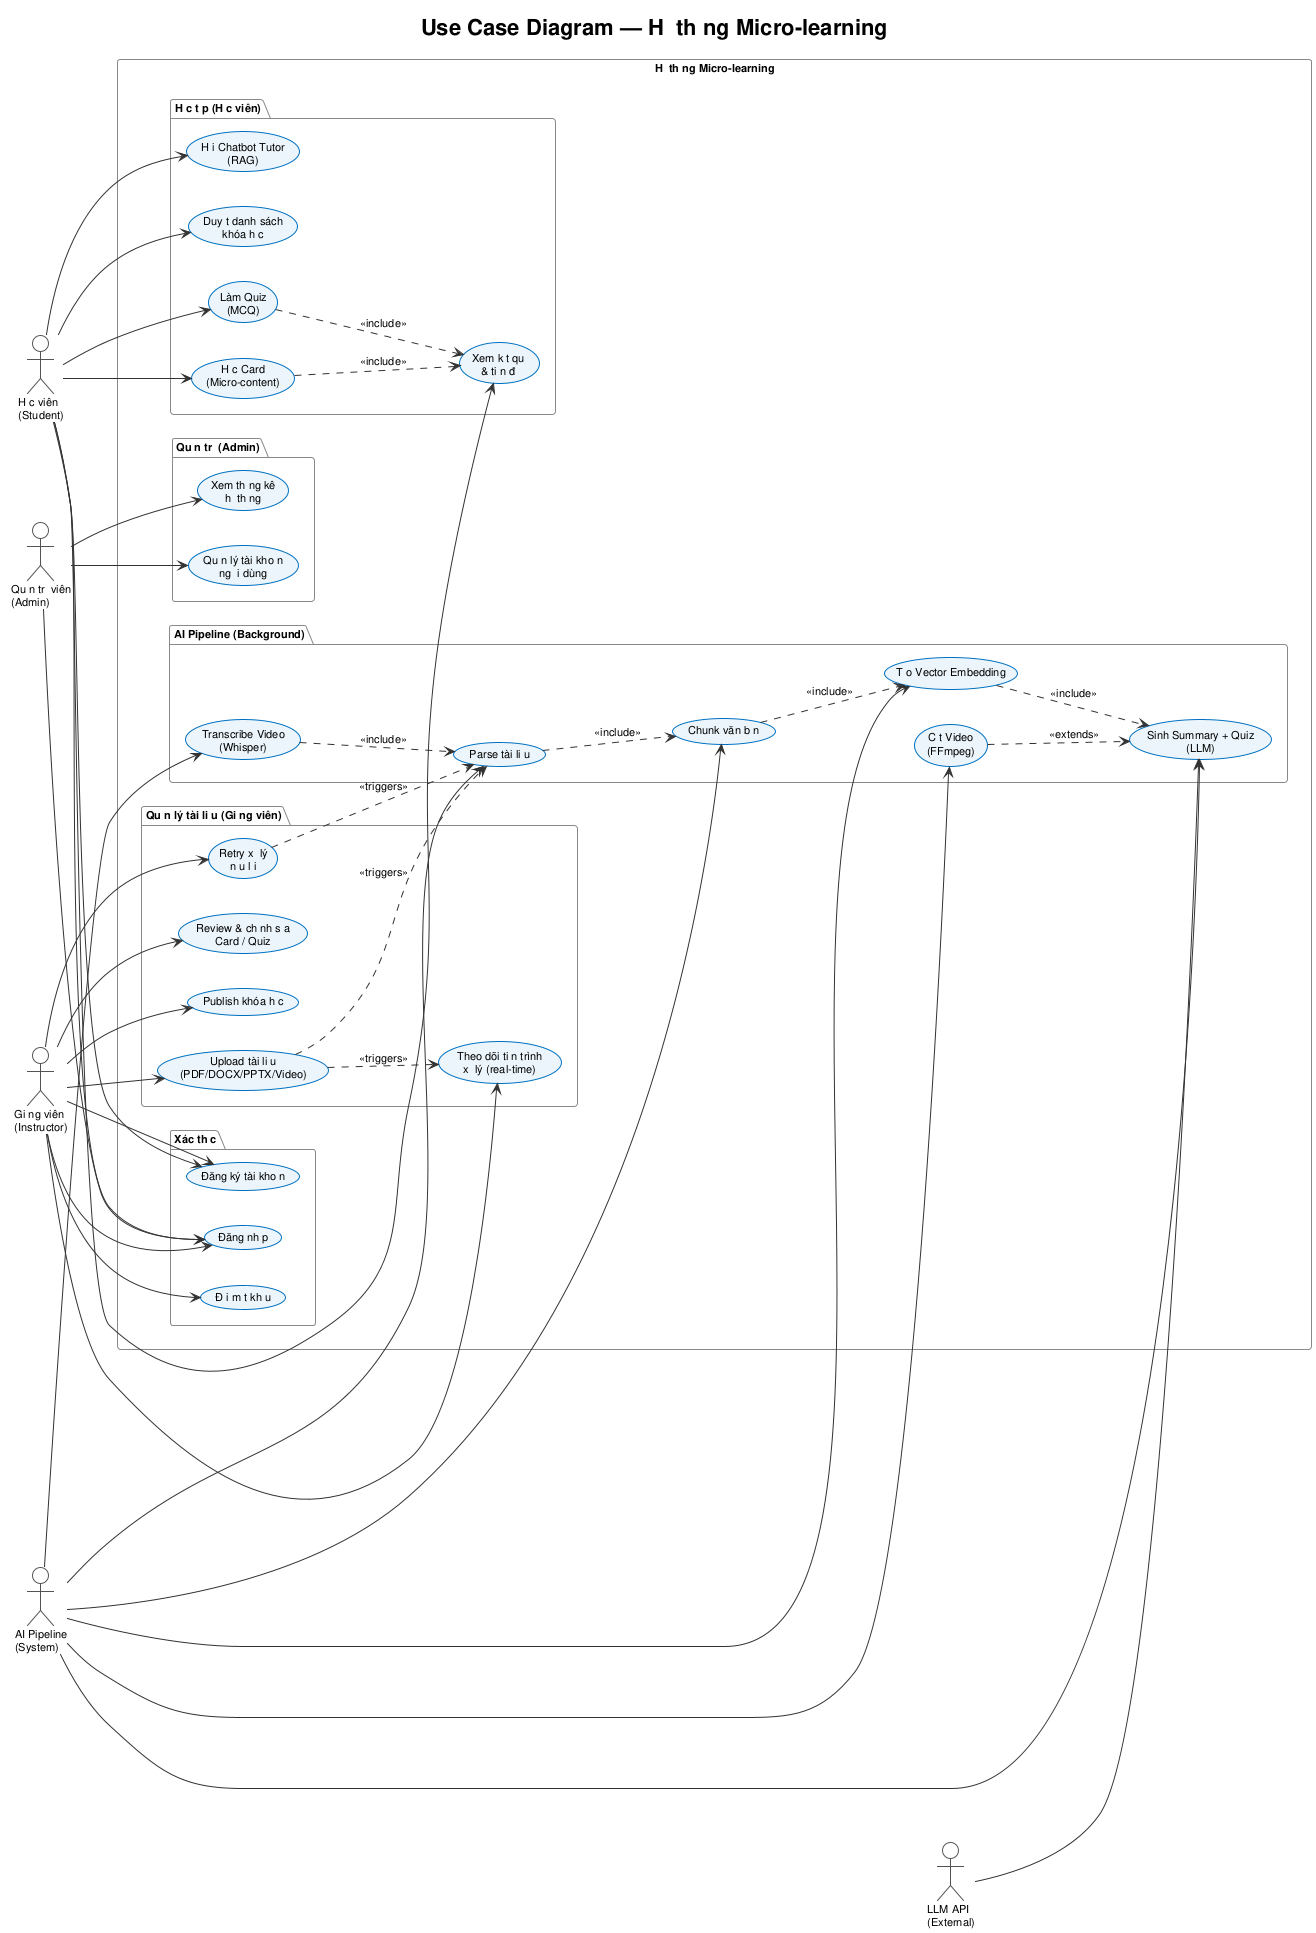
\includegraphics[width=0.88\textwidth,height=0.68\textheight,keepaspectratio]{diagrams/usecase_diagram.png}
    \caption{Use case diagram tổng quát của hệ thống.}
    \label{fig:usecase-diagram-lvtn}
\end{figure}

Các use case chính gồm upload tài liệu, xử lý tài liệu tự động, review nội
dung, publish khóa học, học bằng card, làm quiz, tìm kiếm ngữ nghĩa, ingest
curriculum và quản lý tài khoản. Tác nhân AI Pipeline được mô hình hóa riêng
vì quá trình xử lý diễn ra bất đồng bộ sau khi người dùng upload tài liệu.

\subsection{Đặc tả các Use Case chính}

\subsubsection{UC-01: Upload tài liệu}

\begin{table}[H]
    \centering
    \caption{Thông tin UC-01: Upload tài liệu.}
    \label{tab:uc-upload-lvtn}
    \begin{tabular}{p{3.5cm}p{10.5cm}}
        \toprule
        \textbf{Thuộc tính} & \textbf{Mô tả} \\
        \midrule
        Tác nhân chính & Giảng viên \\
        Tác nhân phụ & AI Pipeline, Object Storage \\
        Mục tiêu & Đưa tài liệu học tập vào hệ thống để bắt đầu pipeline sinh nội dung. \\
        Tiền điều kiện & Giảng viên đã xác thực; khóa học hoặc context LMS đã tồn tại. \\
        Hậu điều kiện & File được lưu, document metadata được tạo, job xử lý được enqueue. \\
        \bottomrule
    \end{tabular}
\end{table}

Luồng chính:
\begin{enumerate}
    \item Giảng viên mở màn hình quản lý tài liệu.
    \item Giảng viên chọn file PDF/DOCX/PPTX và nhập metadata cơ bản.
    \item Frontend kiểm tra định dạng và kích thước.
    \item Backend lưu file vào MinIO và tạo document ở trạng thái
          \texttt{QUEUED}.
    \item Backend enqueue job xử lý tài liệu.
    \item Frontend chuyển sang màn hình theo dõi tiến trình.
\end{enumerate}

Luồng thay thế gồm file sai định dạng, lưu file thất bại hoặc queue tạm thời
không khả dụng. Trong các trường hợp này, hệ thống cần hiển thị lỗi rõ ràng và
cho phép retry khi phù hợp.

\subsubsection{UC-02: Xử lý tài liệu tự động}

\begin{table}[H]
    \centering
    \caption{Thông tin UC-02: Xử lý tài liệu tự động.}
    \label{tab:uc-process-lvtn}
    \begin{tabular}{p{3.5cm}p{10.5cm}}
        \toprule
        \textbf{Thuộc tính} & \textbf{Mô tả} \\
        \midrule
        Tác nhân chính & AI Pipeline \\
        Mục tiêu & Chuyển tài liệu thô thành chunk, embedding, card và quiz. \\
        Tiền điều kiện & File tồn tại trong MinIO; document ở trạng thái \texttt{QUEUED}. \\
        Hậu điều kiện & Document có chunks, vectors, generated cards/quizzes và trạng thái \texttt{DONE}. \\
        \bottomrule
    \end{tabular}
\end{table}

Luồng chính:
\begin{enumerate}
    \item Worker nhận job từ queue.
    \item Worker tải file từ MinIO và chọn parser theo loại file.
    \item Parser trích xuất text, heading và metadata.
    \item Chunker chia tài liệu thành các đơn vị học tập.
    \item Embedder tạo vector và upsert vào Qdrant.
    \item LLM adapter sinh card/quiz cho từng chunk hoặc nhóm chunk.
    \item Metadata store lưu kết quả vào PostgreSQL.
    \item Document chuyển sang \texttt{DONE}.
\end{enumerate}

Luồng thay thế gồm parser lỗi, LLM timeout hoặc Qdrant unavailable. Các lỗi
tạm thời được retry có giới hạn; lỗi cuối cùng được ghi log và chuyển document
sang \texttt{ERROR}.

\subsubsection{UC-03: Review và publish nội dung}

\begin{table}[H]
    \centering
    \caption{Thông tin UC-03: Review và publish nội dung.}
    \label{tab:uc-review-lvtn}
    \begin{tabular}{p{3.5cm}p{10.5cm}}
        \toprule
        \textbf{Thuộc tính} & \textbf{Mô tả} \\
        \midrule
        Tác nhân chính & Giảng viên \\
        Mục tiêu & Kiểm duyệt nội dung do AI sinh ra trước khi học viên truy cập. \\
        Quy tắc nghiệp vụ & Nội dung chưa review không được publish; hệ thống phải lưu dấu vết chỉnh sửa quan trọng. \\
        \bottomrule
    \end{tabular}
\end{table}

Luồng chính:
\begin{enumerate}
    \item Giảng viên mở màn hình review của document đã xử lý.
    \item Hệ thống hiển thị card, quiz, đáp án, giải thích và nguồn chunk.
    \item Giảng viên chỉnh sửa hoặc xóa nội dung chưa phù hợp.
    \item Giảng viên đánh dấu section/document đã review.
    \item Giảng viên publish nội dung cho học viên.
\end{enumerate}

\subsubsection{UC-04: Học bằng card và làm quiz}

\begin{table}[H]
    \centering
    \caption{Thông tin UC-04: Học bằng card và làm quiz.}
    \label{tab:uc-learn-lvtn}
    \begin{tabular}{p{3.5cm}p{10.5cm}}
        \toprule
        \textbf{Thuộc tính} & \textbf{Mô tả} \\
        \midrule
        Tác nhân chính & Học viên \\
        Mục tiêu & Học viên tiếp cận nội dung ngắn, làm câu hỏi kiểm tra và nhận phản hồi. \\
        Dữ liệu lưu & Learning progress, quiz submission, score, timestamp và context bài học. \\
        \bottomrule
    \end{tabular}
\end{table}

Luồng chính:
\begin{enumerate}
    \item Học viên mở bài học từ LMS hoặc trang học tập.
    \item Hệ thống hiển thị danh sách card đã publish.
    \item Học viên đọc card và chuyển sang quiz tương ứng.
    \item Học viên chọn đáp án.
    \item Hệ thống hiển thị đúng/sai, giải thích và lưu kết quả.
\end{enumerate}

\section{Luồng nghiệp vụ chính}

\subsection{Activity Diagrams}

Luồng nghiệp vụ xử lý tài liệu gồm hai nhóm bước chính. Nhóm thứ nhất chuẩn
hóa tri thức từ tài liệu gốc thông qua parse, chunk, embed và persist. Nhóm
thứ hai sinh nội dung học tập thông qua LLM generation, validation và review.
Việc tách hai nhóm bước giúp hệ thống tái sử dụng chunk và embedding cho nhiều
tác vụ khác nhau như search, RAG chatbot hoặc sinh quiz theo Learning Outcome.

\begin{figure}[H]
    \centering
    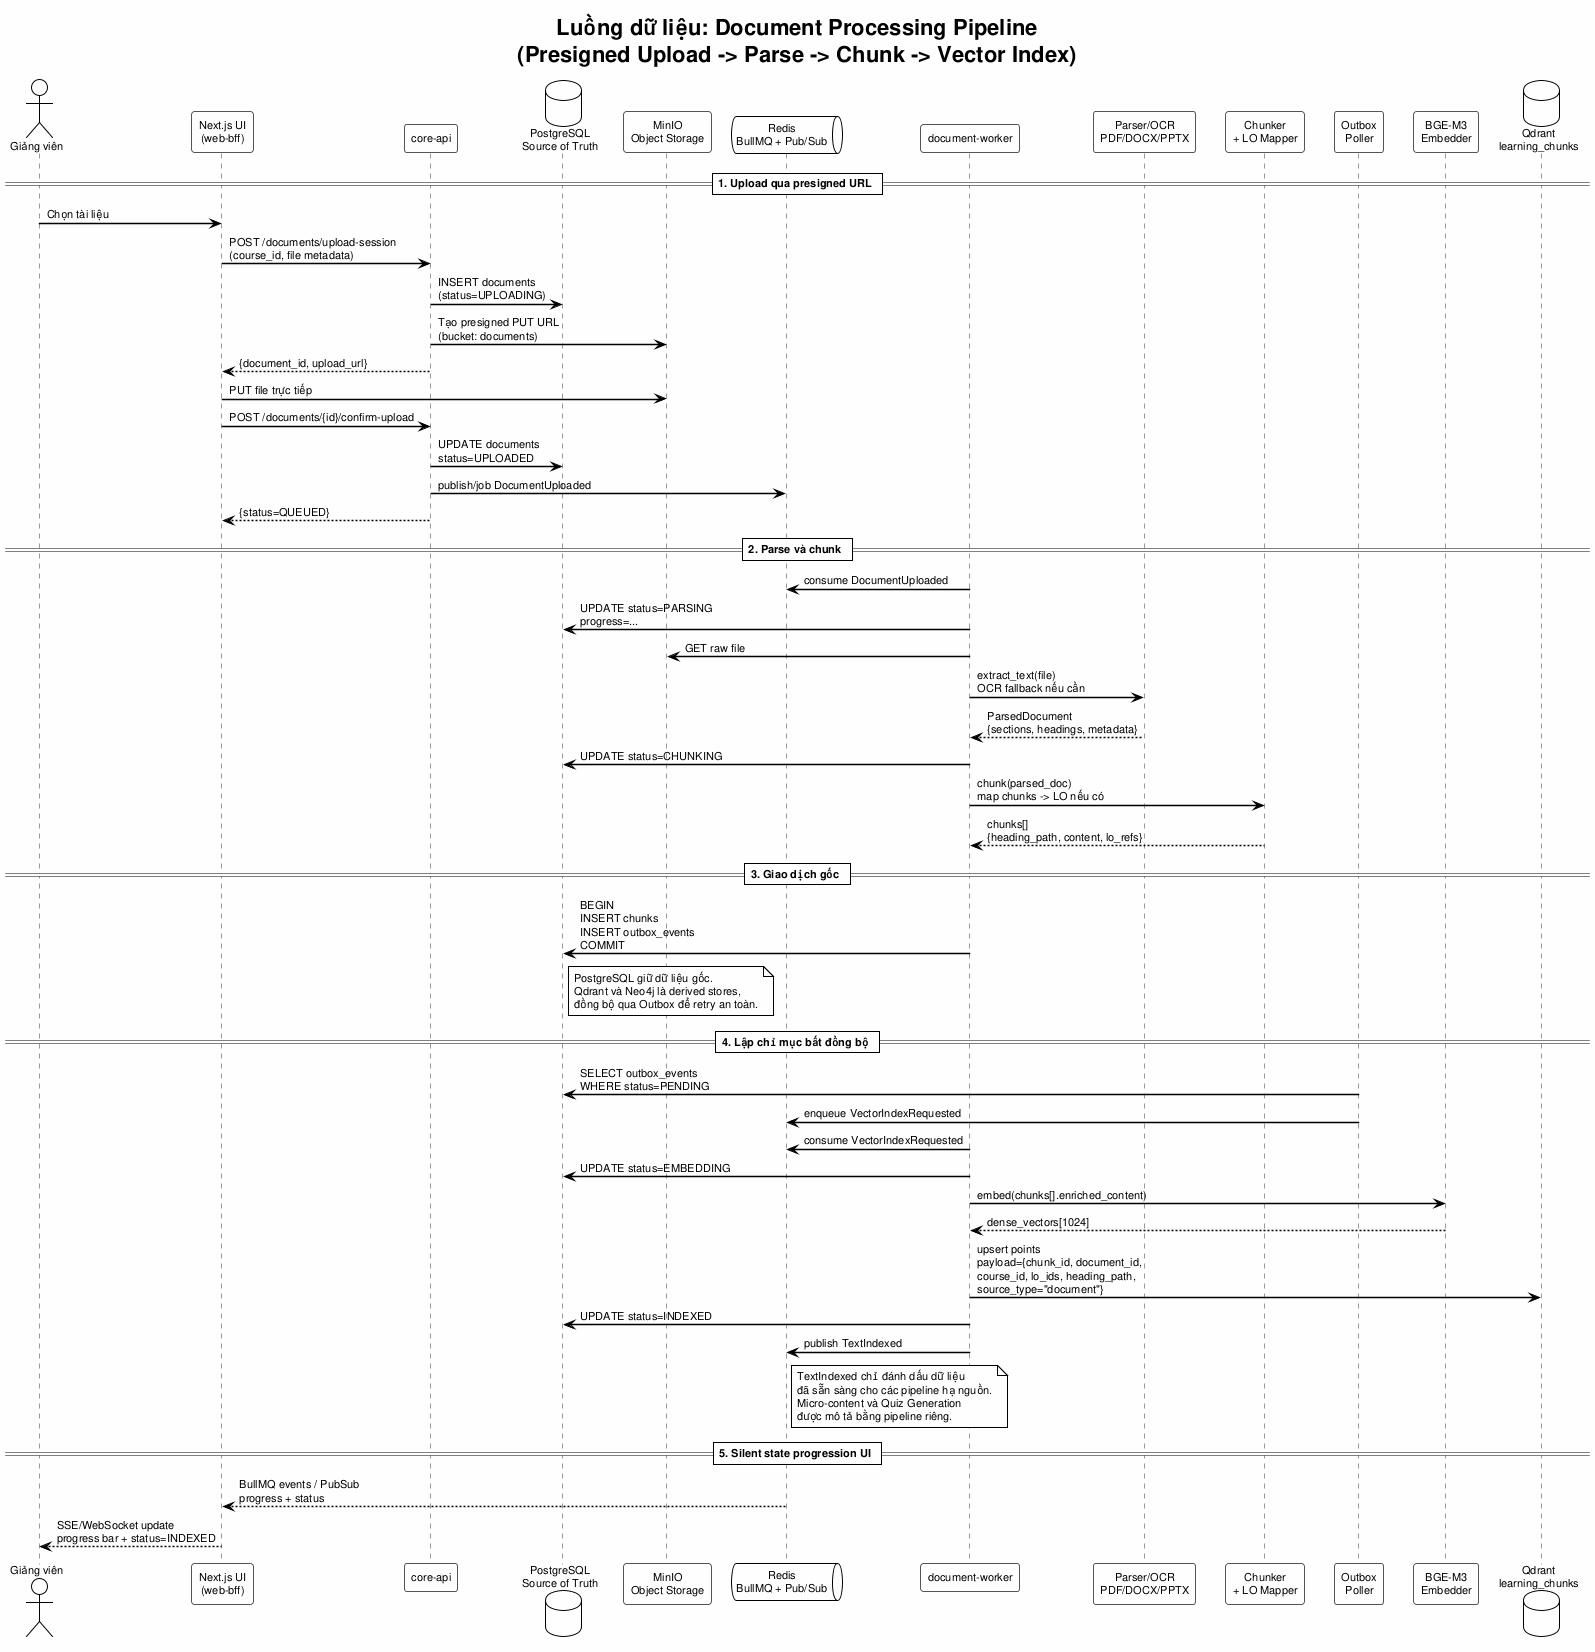
\includegraphics[width=0.92\textwidth]{diagrams/dataflow_text_pipeline.png}
    \caption{Activity/dataflow cho pipeline xử lý tài liệu văn bản.}
    \label{fig:activity-text-pipeline-lvtn}
\end{figure}

\subsection{Dataflow Diagrams}

Luồng RAG bắt đầu từ câu hỏi của học viên hoặc yêu cầu sinh quiz của giảng
viên. Hệ thống tạo embedding cho query, truy xuất chunk liên quan trong
Qdrant, kết hợp metadata và quan hệ trong Knowledge Graph nếu có, sau đó đưa
context vào LLM để sinh câu trả lời hoặc nội dung học tập.

\begin{figure}[H]
    \centering
    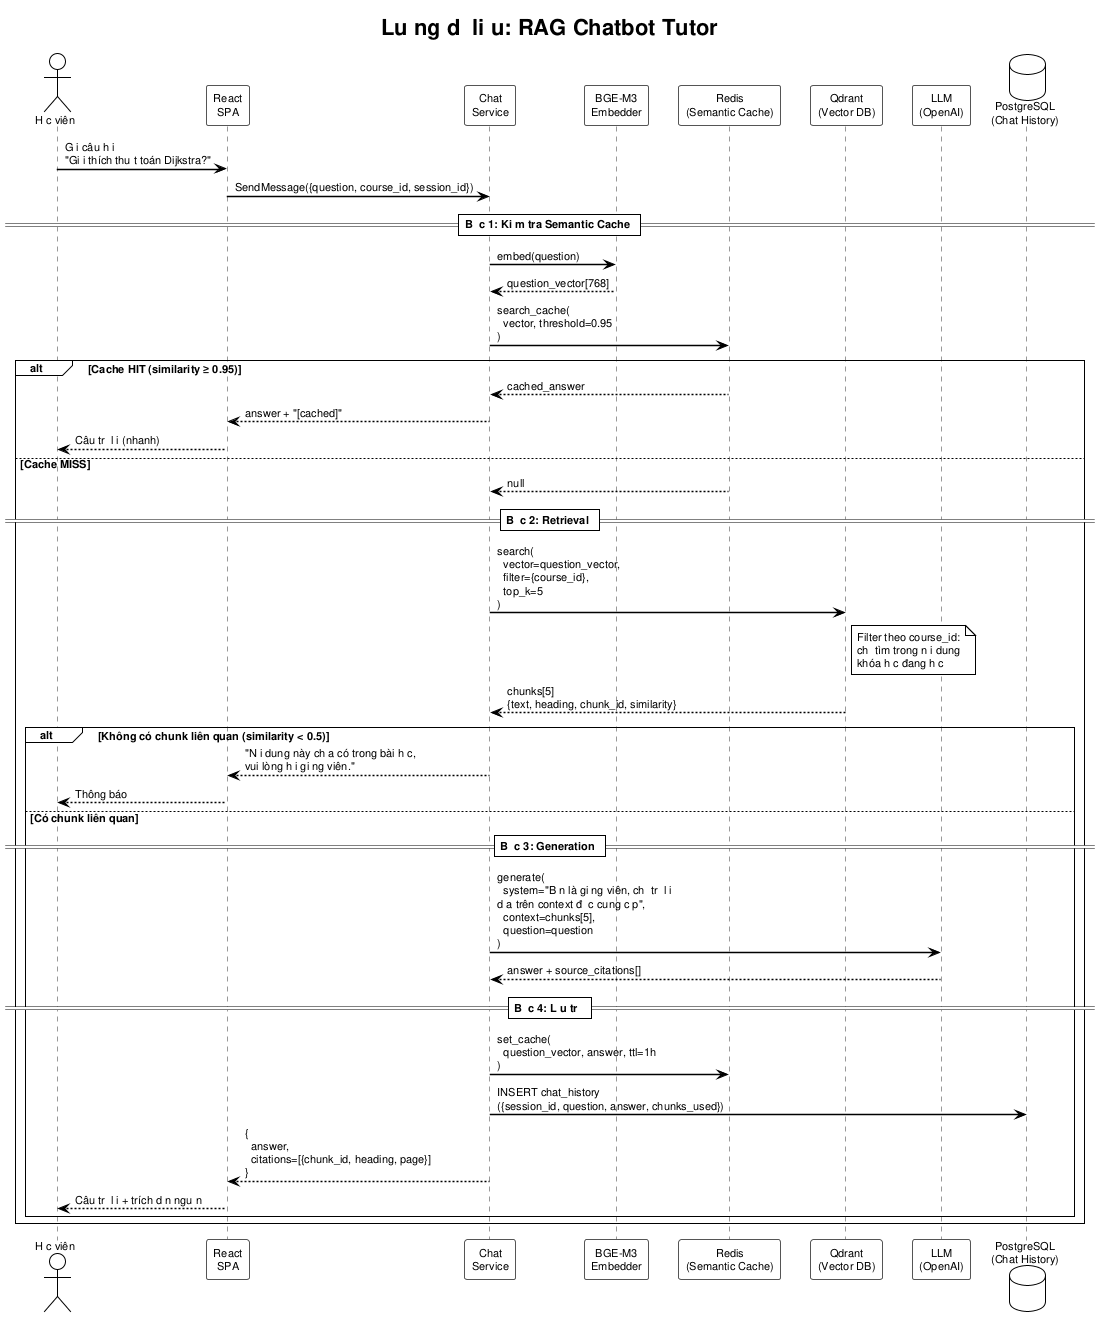
\includegraphics[width=0.92\textwidth]{diagrams/dataflow_rag_chatbot.png}
    \caption{Dataflow cho truy xuất RAG và chatbot học tập.}
    \label{fig:activity-rag-lvtn}
\end{figure}

Các quy tắc nghiệp vụ cần được duy trì trong các luồng trên:
\begin{enumerate}
    \item Học viên chỉ nhìn thấy nội dung đã publish.
    \item Nội dung AI sinh ra phải có nguồn liên kết đến document/chunk gốc.
    \item Quiz sinh theo LO phải lưu LO code, Bloom level và rationale nếu có.
    \item Job xử lý tài liệu phải có trạng thái cuối rõ ràng: \texttt{DONE}
          hoặc \texttt{ERROR}.
    \item Lỗi LLM hoặc vector DB không được làm mất document gốc.
    \item LTI launch phải xác thực trước khi tạo session học tập.
\end{enumerate}
